\documentclass[english,12pt]{beamer}

\usepackage{mathptmx,amsmath,amssymb,graphicx,bibentry,bbm,babel,ragged2e}

\makeatletter

\newcommand{\noun}[1]{\textsc{#1}}
\newcommand{\jitem}[1]{\item \begin{justify} #1 \end{justify} \vfill{}}
\newcommand{\sframe}[2]{\frame{\frametitle{#1} #2}}

\newenvironment{centercolumns}{\begin{columns}[c]}{\end{columns}}
%\newenvironment{jitem}{\begin{justify}\begin{itemize}}{\end{itemize}\end{justify}}

\usetheme{Warsaw}
\setbeamertemplate{footline}[text line]{}
\setbeamercolor{structure}{fg=purple!50!blue, bg=purple!50!blue}

\setbeamercovered{transparent}


\@ifundefined{showcaptionsetup}{}{%
 \PassOptionsToPackage{caption=false}{subfig}}
\usepackage{subfig}
\makeatother

\begin{document}


\title{Models Coupling Urban Growth and Transportation Network Growth : An Algorithmic Systematic Review Approach}

\author{J.~Raimbault$^{1,2}$\\
\texttt{juste.raimbault@polytechnique.edu}
}


\institute{$^{1}$UMR CNRS 8504 G{\'e}ographie-cit{\'e}s\\
$^{2}$UMR-T IFSTTAR 9403 LVMT\\
}


\date{ECTQG 2015 Bari\\
Parallel Session : new data, methods\\
September 7, 2015}

\frame{\maketitle}


%%%%%%%%%%%%%%%%%
\section{Introduction}
%%%%%%%%%%%%%%%%%


%%%%%%%%%%%%%%%%%
\subsection{Introduction}
%%%%%%%%%%%%%%%%%


%%%%%%%%%%%%%%%%%
\sframe{Lost in Translation}{

Science is all about \emph{perspective}~\cite{giere2010scientific}...

\smallskip

Antagonist perspectives ?

\smallskip

\noun{G. Caruso} saturday : Spatial ABM and Urban economy should (have to) reconciliate !

but even economist disagree~\cite{marchionni2004geographical} : geo. eco. \textit{vs} eco. geo.

\smallskip

\textit{Listen to your teachers !}

\noun{F. Leurent} : your traffic model is wrong because out-of-eq.

\noun{M. Barthelemy} : now we build a rigorous ``urban science'', all existing modeling work is garbage.

\smallskip

\textit{That escalated quickly...} scientific aggressivity !~\cite{dupuy2015sciences}

$\rightarrow$ Do we ``really stand together'' ?~\cite{pavlidis2014together}

}
%%%%%%%%%%%%%%%%%%%%%%%%%%%%

%%%%%%%%%%%%%%%%%
\subsection{Problematic}
%%%%%%%%%%%%%%%%%



%%%%%%%%%%%%%%%%%
\sframe{Research context}{

Thematic framework of the study of \emph{transportation-cities (land-use) interactions}, on which misleading conceptions dominate~\cite{offner1993effets}. 

\bigskip

\cite{bretagnolle:tel-00459720} draws powerful empirical conclusions and claims for a need of \textbf{modeling the co-evolution process}.


\bigskip

$\rightarrow$ \textit{State-of-the-art of such an hybrid modeling ?}


\bigskip

{\textit{Disclaimer : NOT a thematic presentation on network/urban coevolution but more an applied epistemological study.}}

}
%%%%%%%%%%%%%%%%%%%%%%%%%%%%





%%%%%%%%%%%%%%%%%
\sframe{Brief Litterature Review}{

\begin{itemize}
\jitem{LUTI approaches : transport integrated but static network (reviews : \cite{chang2006models,iacono2008models}\\\cite{wegener2004land}). Various refinements (e.g. \\\cite{delons:hal-00319087} housing market), many aspects can be taken into account~\cite{wegener1991one}}
\jitem{Network Growth : Economic network growth~\\\cite{zhang2007economics,xie2009modeling} ;\\
Physical approaches~\cite{barthelemy2008modeling} ;\\
Biological self-organizing network~\cite{TeroAl10}.}
\jitem{Hybrid dynamic approaches : few works propose dynamic coupled models, always toy-models. \cite{DBM11,MBB09}\cite{schmitt2014modelisation}\cite{raimbault2014hybrid}\\\cite{le2015modeling}}
\end{itemize}

}
%%%%%%%%%%%%%%%%%%%%%%%%%%%%



%%%%%%%%%%%%%%%%%
\sframe{Research questions}{


\textbf{Primal research question : }

\medskip

\textit{Why so few contributions on modeling this crucial problem ? What could be the role of the well-known disciplinar compartmentalization on that issue ?}

\bigskip

\textbf{Dual research question : }

\medskip

\textit{How does lack of pluridisciplinarity influences scientific outcomes ? Can this be understood through quantitative epistemology analyses ?}

}
%%%%%%%%%%%%%%%%%%%%%%%%%%%%






%%%%%%%%%%%%%%%%%
\sframe{Work hypothesis}{

\textbf{Possible Explanations : }
\begin{itemize}
\jitem{Too difficult problem ? (Fear of negative results~\cite{ioannidis2005most}). ``\textit{A tale of complex coupling of spatio-temporal socio-technical processes at the good scales}'' : Good luck !}
\jitem{Tried before (a long time ago) and forget ?\\\cite{rey2015these}}
\jitem{Compartmentalization of disciplines having different ontological frameworks, research objectives, etc.\\\cite{commenges:tel-00923682}}
\end{itemize}

\medskip

$\rightarrow$ Work on testing quantitatively the last hypothesis.




}
%%%%%%%%%%%%%%%%%%%%%%%%%%%%






%%%%%%%%%%%%%%%%%
\section{Methods}
%%%%%%%%%%%%%%%%%


%%%%%%%%%%%%%%%%%
\sframe{Proposed approach}{

\textit{Bibliometric quantitative analysis}

\begin{itemize}
\jitem{Bibliometry and Systematic Reviews (SR) play nowadays a significant role in many disciplines (see SR/Meta-Analyses in therapeutic evaluation~\cite{rucker2012network}) ; 11 SR.day$^{-1}$ \cite{10.1371/journal.pmed.1000326} !}
\jitem{SR may even be considered as mandatory as missing a reference is more a mistake given new ressources~\cite{lissacksubliminal}.}
\jitem{Interesting results such as models predicting success of a paper and scientific success~\cite{Wang04102013}}
\jitem{Current bibliometric network study do rely on citation networks~\cite{2013arXiv1310.8220N} or co-autorship networks~\cite{2014arXiv1402.7268S}}
\end{itemize}


}
%%%%%%%%%%%%%%%%%%%%%%%%%%%%

%%%%%%%%%%%%%%%%%
\sframe{Proposed approach}{

$\rightarrow$ \textit{Iterative construction of semantic neighborhoods in scientific reference network.}

\begin{itemize}
\jitem{Extension of the method proposed in~\cite{chavalarias2013phylomemetic} where a dynamic cartography of scientific disciplines is built through text-mining (\emph{phylomemy}).}
\jitem{Based on generalized keywords extraction from titles and abstracts of references, we propose to iteratively explore the keyword co-occurence network.}
\jitem{If disciplines are indeed ``closed'', we should converge towards communities.}
\end{itemize}


}
%%%%%%%%%%%%%%%%%%%%%%%%%%%%



%%%%%%%%%%%%%%%%%
\sframe{Algorithm formalization}{

Let $\mathcal{A}$ an alphabet, $\mathcal{A}^{\ast}$ words and $\mathcal{T}=\cup_{k\in \mathbb{N}}{\mathcal{A}^{\ast}}^k$ finite texts on it ; set of references at iteration $n$ denoted $\mathcal{C}_{n}\in \mathcal{T}^3$. Set of keywords $\mathcal{K}_n$, initial keywords $\mathcal{K}_0$

\medskip

\textbf{Iteration of the algorithm}
\begin{itemize}
\item Intermediate corpus $\mathcal{R}_n$ is obtained through a catalog request from previous keywords $\mathcal{K}_{n-1}$.
\item New corpus :  $\mathcal{C}_n = \mathcal{C}_{n-1} \cup \mathcal{R}_n$.
\item New keywords $\mathcal{K}_n$ extracted from corpus through Natural Language Processing, with $N_k$ fixed number of keywords.
\end{itemize}

\textbf{Stopping criteria} : converged corpus size or fixed max iteration


}
%%%%%%%%%%%%%%%%%%%%%%%%%%%%



%%%%%%%%%%%%%%%%%
\sframe{Algorithm architecture}{
% figure

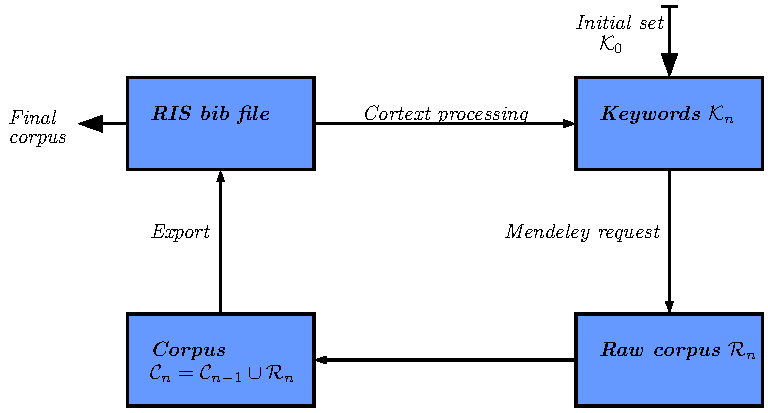
\includegraphics[width=\textwidth]{figures/schema_algo.pdf}


}
%%%%%%%%%%%%%%%%%%%%%%%%%%%%



%%%%%%%%%%%%%%%%%
\sframe{Convergence : sketch of proof}{
\textbf{1st attempt : } we have obviously, with $K,C$ keyword extraction and catalog request functions, $|\mathcal{C}_n|\leq |\mathcal{C}_{n+1}|\leq |\mathcal{C}_n| + |C[K(\mathcal{C}_n)]|$, what gives $|C[K(\mathcal{C}_n)]|\rightarrow 0\iff |\mathcal{C}_n| \textrm{ bounded} \iff \mathcal{C}_n\textrm{ converges}$. \textit{But assumptions difficultly interpretable}

\medskip

\textbf{2nd attempt : }
\begin{itemize}
\jitem{Assumption 1 : existence of \emph{communities} $\mathcal{S}$ in network, on which $K$ is stable.}
\jitem{Assumption 2 : \emph{random} steering behavior of the corpus (if not, converges as it growths)}
\jitem{Then $T = \inf_n \mathcal{C}_n \in \mathcal{S}$ is a Stopping Time and thus convergence by stability of any $S\in \mathcal{S}$.}
\end{itemize}

}
%%%%%%%%%%%%%%%%%%%%%%%%%%%%



%%%%%%%%%%%%%%%%%
\sframe{Implementation}{
$\rightarrow$\textit{Heterogeneity of functional specifications suggest an hybrid architecture (applied language agnosticity !) : }
\medskip
\begin{itemize}
\jitem{Core implemented in java ; experiment module in R}
\jitem{Catalog request done to Mendeley open catalog~\cite{mendeley} through REST API.}
\jitem{Natural Language Processing through an hacked API of the web platform provided openly by~\cite{chavalarias2013phylomemetic} in the frame of the \emph{Cortext} project.}
\end{itemize}

\medskip

\textit{Openly available at\\\texttt{https://github.com/JusteRaimbault/CityNetwork/tree/}\\\texttt{master/Models/Biblio/AlgoSR/AlgoSRJavaApp}}

}
%%%%%%%%%%%%%%%%%%%%%%%%%%%%



%%%%%%%%%%%%%%%%%
\section{Results}
%%%%%%%%%%%%%%%%%


%%%%%%%%%%%%%%%%%
\subsection{Validation}
%%%%%%%%%%%%%%%%%


%%%%%%%%%%%%%%%%%
\sframe{Algorithm convergence}{

\textit{Influence of parameters on convergence behavior}

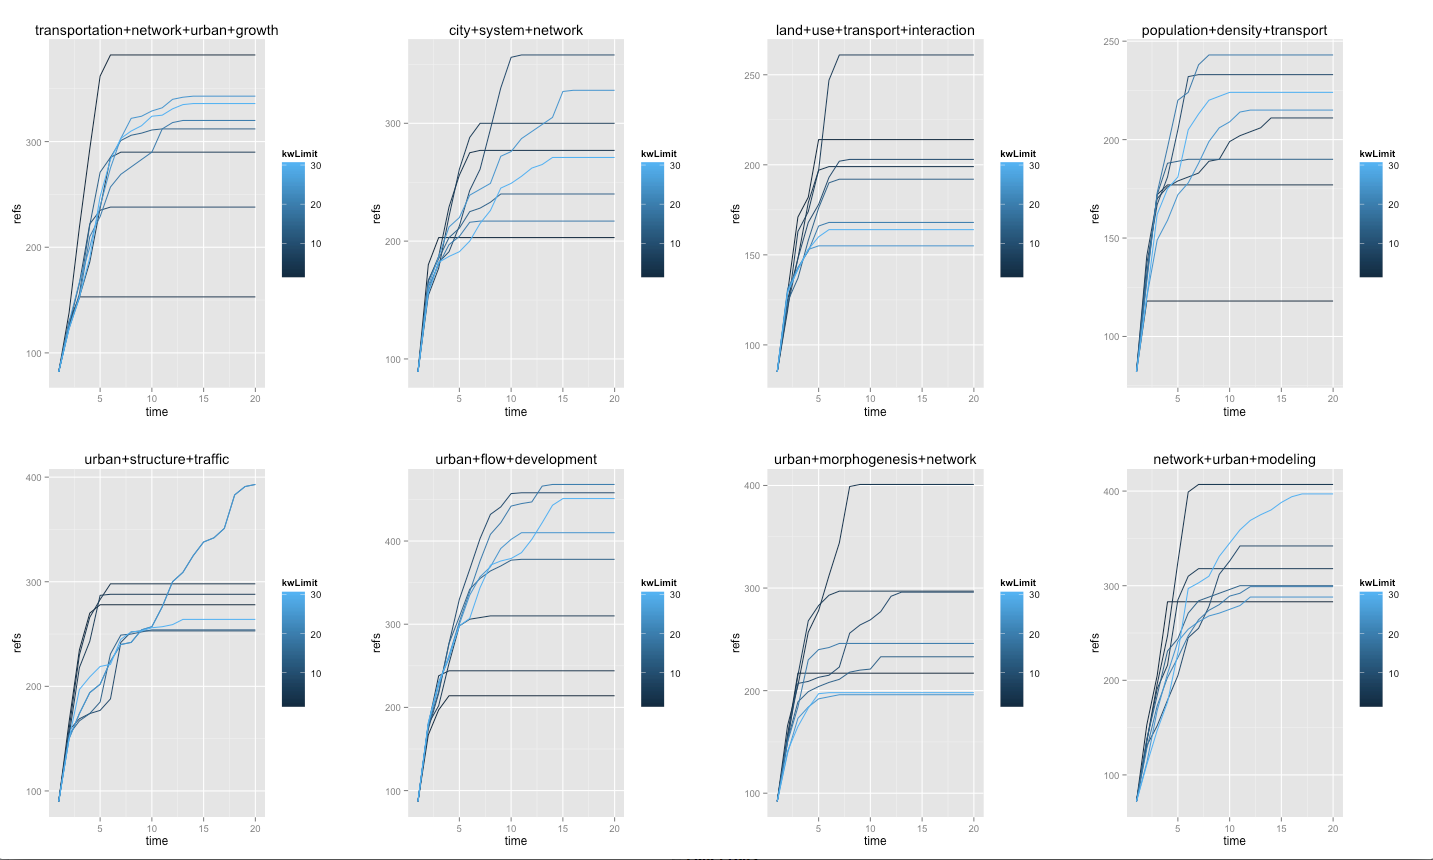
\includegraphics[width=\textwidth]{figures/explo.png}


}
%%%%%%%%%%%%%%%%%%%%%%%%%%%%

%%%%%%%%%%%%%%%%%
\sframe{Algorithm consistence}{

\textit{Corpus lexical consistence}

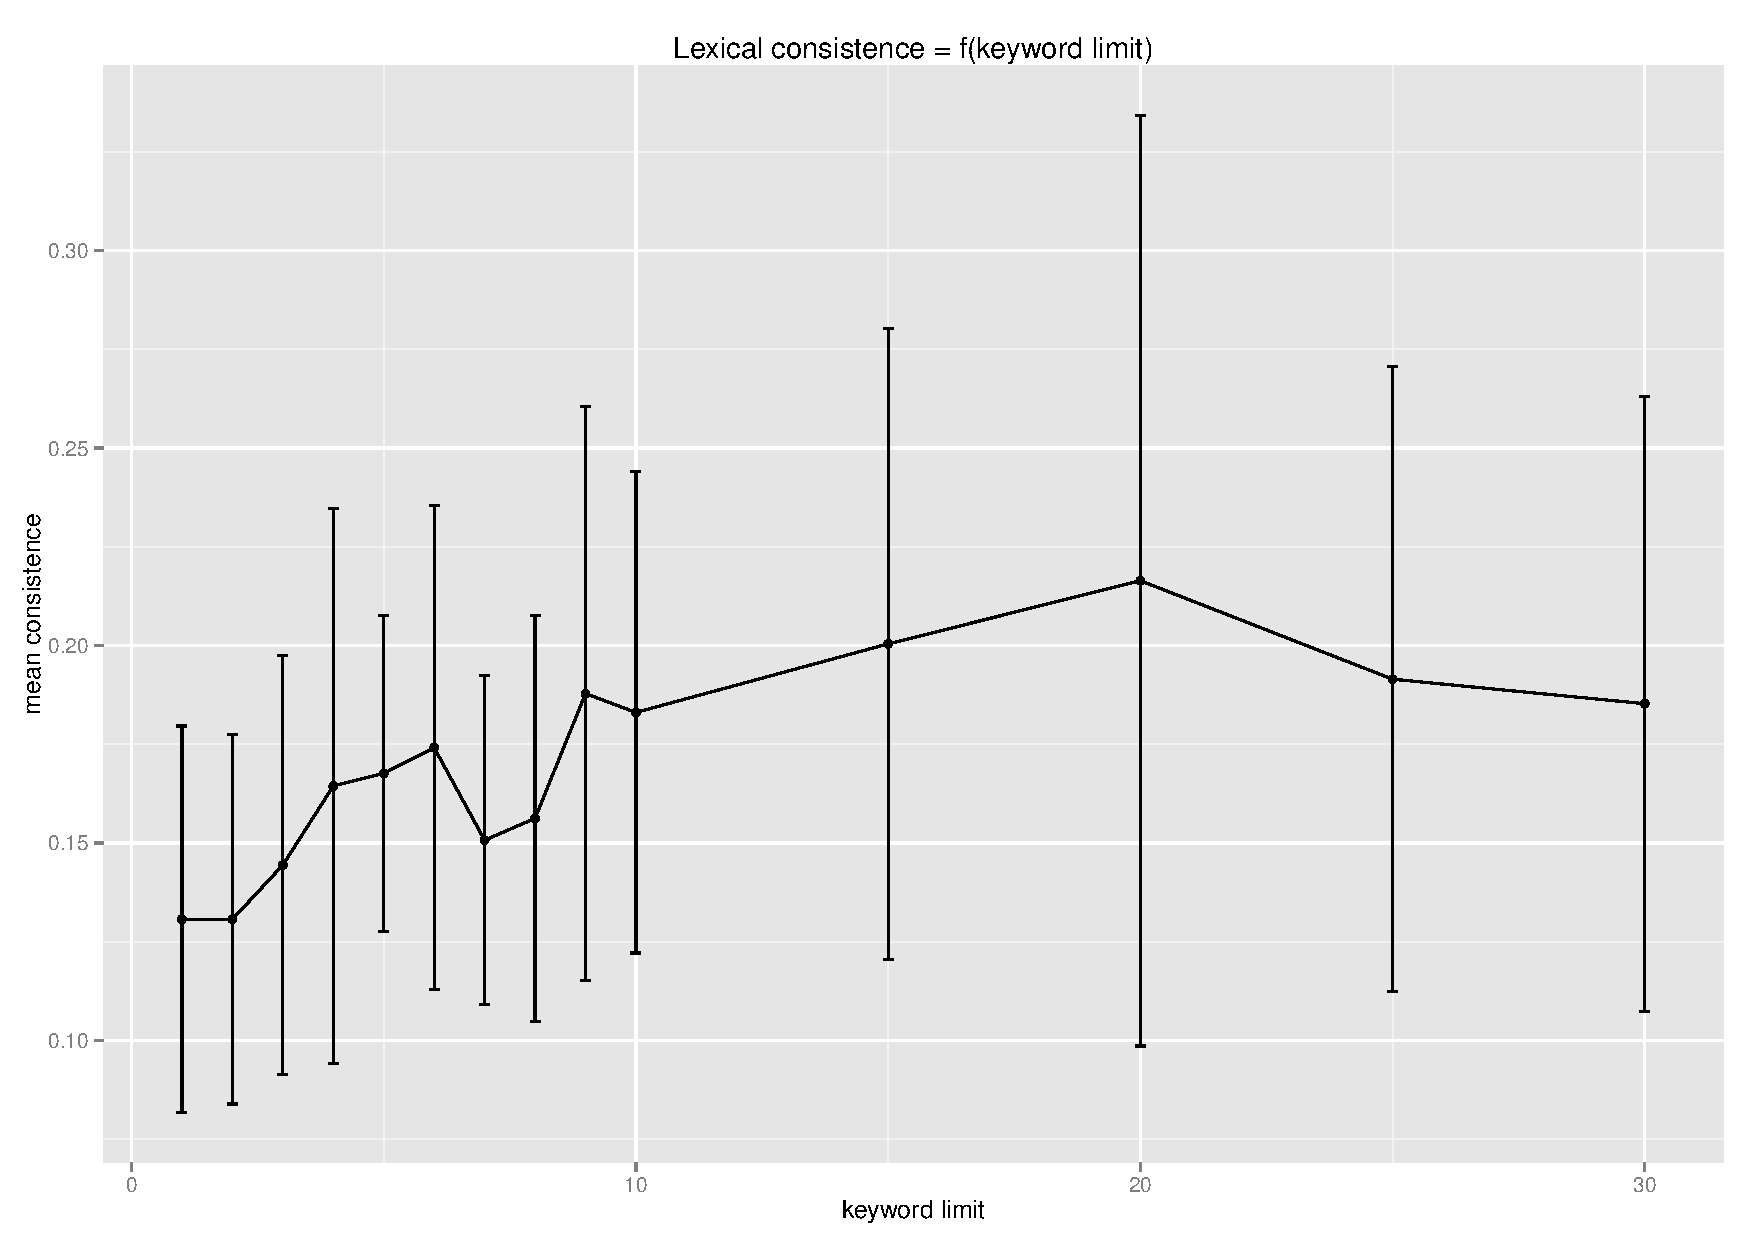
\includegraphics[width=0.9\textwidth]{figures/lexicalConsistence_MeanSd}


}
%%%%%%%%%%%%%%%%%%%%%%%%%%%%




%%%%%%%%%%%%%%%%%
\subsection{Application}
%%%%%%%%%%%%%%%%%


%%%%%%%%%%%%%%%%%
%\sframe{Application : corpus network}{
%
%
%}
%%%%%%%%%%%%%%%%%%%%%%%%%%%%


%%%%%%%%%%%%%%%%%
\sframe{Application : experimental design}{


$\rightarrow$ \textbf{Initial entries :} \texttt{city+system+network}, \texttt{land+use+transport+interaction}, \texttt{network+urban+modeling}, \texttt{population+density+transport}, \texttt{transportation+network+urban+growth}

\medskip

$\rightarrow$ \textbf{Not restraining propagation parameter : } $N_k = 30$

\medskip

$\rightarrow$ \textbf{Large convergence time} (obtained convergence steps : 16, 8, 17, 14,14)

}
%%%%%%%%%%%%%%%%%%%%%%%%%%%%



%%%%%%%%%%%%%%%%%
\sframe{Application : corpuses distances}{
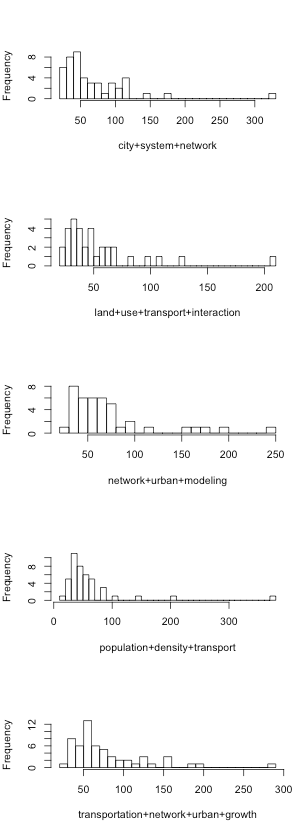
\includegraphics[width=0.2\textwidth,height=0.8\textheight]{figures/hists_corpuses_dists.png}
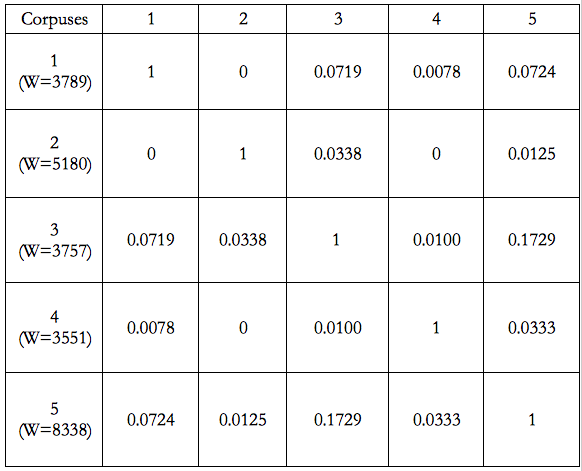
\includegraphics[width=0.8\textwidth]{figures/tab.png}
}
%%%%%%%%%%%%%%%%%%%%%%%%%%%%




%%%%%%%%%%%%%%%%%
\sframe{Application : ongoing extensions}{

\begin{enumerate}
\jitem{Method of construction of controlled random synthetic corpuses, to construct a kind of \emph{null model} to have objective benchmark on intercluster rates.}
\jitem{Comparison of results obtained by semantic analysis with results from citation network or co-authorship network ; should find similar patterns.

\textit{Problem : } Construction of citation network from \textbf{Open Data} is tricky ; elaboration of a scholar API avoiding google blocking using a TOR threads pool.}
\end{enumerate}

}
%%%%%%%%%%%%%%%%%%%%%%%%%%%%






%%%%%%%%%%%%%%%%%
\section{Discussion}
%%%%%%%%%%%%%%%%%

%%%%%%%%%%%%%%%%%
\subsection{Discussion}
%%%%%%%%%%%%%%%%%




%%%%%%%%%%%%%%%%%
\sframe{Discussion}{
\begin{itemize}
\jitem{Quality of / robustness to catalog~\cite{bohannon2014scientific} has to be more investigated.}
\jitem{``Subjective'' initial review and corpuses choices should be more systematically based on expert knowledge.}
\jitem{More systematic analysis and exploration of behavior, as for a computationnal model (concept of proof in Social Sciences ?~\cite{banos2013pour}\cite{laughlin2006different}}
\jitem{Need to use/implement analysis and visualization tools such as in~\cite{cuyala2015geographer}}
\end{itemize}
}
%%%%%%%%%%%%%%%%%%%%%%%%%%%%



%%%%%%%%%%%%%%%%%
\subsection{Perspectives}
%%%%%%%%%%%%%%%%%


%%%%%%%%%%%%%%%%%
\sframe{Perspectives}{
\begin{itemize}
\jitem{Project of a qualitative work (interviews of ``old'' experts, archives, grey litterature investigation) following the methodology of~\cite{commenges:tel-00923682}.}
\jitem{Algorithm as an Open source software available, easy to use by anybody $\implies$ perspective of data collection on algorithm behavior ; collaborative building of local science maps from expert knowledge.}
\jitem{Transposition of the methodology in other bibliometrical projects.}
\end{itemize}
\medskip
\textbf{Conclusion : } Proposition and implementation of an iterative semantic discipline mapping algorithm ; first results suggest a positive answer to the compartmentalization hypothesis.
}
%%%%%%%%%%%%%%%%%%%%%%%%%%%%





%%%%%%%%%%%%%%%%%
\sframe{Reserve slides}{

\textbf{Reserve Slides}

}
%%%%%%%%%%%%%%%%%%%%%%%%%%%%



%%%%%%%%%%%%%%%%%
\sframe{Lexical consistence}{


Lexical consistence is defined though co-occurrences of keywords by, with $N$ final number of keywords, $f$ final step, and $c(i)$ co-occurrences in references, $\kappa = \frac{2}{N(N-1)}\sum_{i,j \in \mathcal{K}_f}{|c(i)-c(j)|}$



}
%%%%%%%%%%%%%%%%%%%%%%%%%%%%



%%%%%%%%%%%%%%%%%
\sframe{Corpuses Distances}{


Corpus distances defined as

\[
d(i,j) = \frac{\sum_{k,l} \mathbbm{1}_{w_{ki}=w_{lj}}\cdot (c_{ki}+c_{lj})}{\sum_k{(c_{ki} + c_{kj})}}
\]



}
%%%%%%%%%%%%%%%%%%%%%%%%%%%%




%%%%%%%%%%%%%%%%%%%%%
\begin{frame}[allowframebreaks]
\frametitle{References}
\bibliographystyle{apalike}
\bibliography{/Users/Juste/Documents/ComplexSystems/CityNetwork/Biblio/Bibtex/CityNetwork,/Users/Juste/Documents/ComplexSystems/Biblio/Culture/Culture/culture,biblio,/Users/Juste/Documents/ComplexSystems/Conferences/ICCSS2015/Biblio/iccss2015}
\end{frame}
%%%%%%%%%%%%%%%%%%%%%%%%%%%%












\end{document}















